\documentclass[11pt]{article}
 
\usepackage[margin=.95in]{geometry} 
\usepackage{amsmath,amsthm,amssymb, graphicx, multicol, array}
 
\newcommand{\N}{\mathbb{N}}
\newcommand{\Z}{\mathbb{Z}}
 

\begin{document}
 
\title{Homework 1}
\author{Juliette Franqueville\\
}
\maketitle

\section*{(1) Prove Slutsky's theorem.}

Slutsky's theorem states that 

\begin{itemize}
\item $x_n \xrightarrow[]{P} x \Rightarrow x_n \xrightarrow[]{D} x$
\item $x_n \xrightarrow[]{D} x_0 \Rightarrow x_n \xrightarrow[]{P} x_0$
    \item if $x_n \xrightarrow[]{D} x$ and $z_n \xrightarrow[]{P} z_0$, then 
\end{itemize}
 
\begin{align*}
    x_n +z_n &\xrightarrow[]{D} x+z_0\\
    x_n z_n &\xrightarrow[]{D} xz_0\\
    x_n / z_n &\xrightarrow[]{D} x/z_0\\
\end{align*}

We will prove the three lemmas in order. 

First, we have to show that if $x_n \xrightarrow[]{P} x$,   $\lim_{n \to \infty }Pr(x_n \leq a)  = Pr(x \leq a)$ for any $a$. 


We show, using basic probability rules, that for $\epsilon > 0$

\begin{align*}
Pr(x_n \leq a) &= Pr(x_n \leq a, x \leq a + \epsilon) + Pr(y > a, x \leq a + \epsilon)\\
& \leq Pr(x \leq a + \epsilon) + Pr(x_n - x > a-x, a-x<-\epsilon)\\
& \leq Pr(x \leq a + \epsilon) + Pr(x_n - x <-\epsilon)\\
& \leq Pr(x \leq a + \epsilon) + Pr(x_n - x <-\epsilon)+ Pr(x_n - x > \epsilon)\\
& \leq Pr(x \leq a + \epsilon) + Pr(|x_n - x| > \epsilon)\\
\end{align*}

So, 

\begin{align*}
Pr(x_n \leq a) &\leq Pr(x \leq a + \epsilon) + Pr(|x_n - x| > \epsilon)\\
Pr(x_n \leq a-\epsilon) &\leq Pr(x \leq a) + Pr(|x_n - x| > \epsilon)\\
Pr(x_n \leq a-\epsilon) -Pr(|x_n - x|) > \epsilon)&\leq Pr(x_n \leq a)  \leq Pr(x_n \leq a+\epsilon) +Pr(|x_n - x|>\epsilon)
\end{align*}

Taking the limit as $n \to \infty$, we find that
$F_x(a-\epsilon) \leq \lim_{n \to \infty } Pr(x_n \leq a) \leq F_x(a+\epsilon)$, so (from the squeeze theorem), $\lim_{n \to \infty }Pr(x_n \leq a)  = Pr(x \leq a)$ as $\epsilon \to 0$.\\

Secondly, we have to show that if $x_n \xrightarrow[]{D} x_0$,  $\lim_{n \to \infty }P(|x_n -x| > \epsilon) = 0$. We have:

\begin{align*}
    \lim_{n \to \infty }P(|x_n-x_0| \leq \epsilon) &=   \lim_{n \to \infty } P(-\epsilon\leq x_n-x_0 \leq \epsilon)\\
    &=  \lim_{n \to \infty }P(x_n-x_0 \leq \epsilon) - \lim_{n \to \infty }P(x_n-x_0 \leq - \epsilon)\\
    &=  \lim_{n \to \infty }P(x_n \leq \epsilon+x_0) - \lim_{n \to \infty }P(x_n \leq x_0 - \epsilon)\\
      &=  \lim_{n \to \infty }F_{xn}(\epsilon+x_0) - \lim_{n \to \infty }F_{xn}(x_0-\epsilon) \\ &= 1-0=1\\
\end{align*}

Or, equivalently,  $\lim_{n \to \infty }P(|x_n -x_0| > \epsilon) = 0$; which is the definition of convergence in probability. To go from the second to last to the last line, we used the fact that $x_n \xrightarrow[]{D} x_0$. \\




We know that if $z_n \xrightarrow[]{P} z_0$, $z_n \xrightarrow[]{D} z_0$. Lastly, we show that $(x_n, z_n)\xrightarrow[]{D} (x, z_0)$.  If $(x_n, z_0) \xrightarrow[]{D} (x, z_0)$ and $(x_n, z_n) - (x_n, z_0) \xrightarrow[]{P} 0$, then $(x_n, z_n) \xrightarrow[]{D} (x, z_0)$.  $(x_n, z_0) \xrightarrow[]{D} (x, z_0)$  follows from the continuous mapping theorem, and $(x_n, z_n) - (x_n, z_0) = z_n - z_0 \xrightarrow[]{P} 0$, so  $(x_n, z_n) \xrightarrow[]{D} (x, z_0)$. We then simply use the continuous mapping theorem:

\begin{align*}
    x_n & \xrightarrow[]{D} x \\ 
    g(x_n) & \xrightarrow[]{D} g(x) \\ 
\end{align*}

with $g(x,y) = x+y$,  $g(x,y) = xy$, and $g(x,y) = x/y$ to prove the last part of Slutsky's theorem.


\section*{(2) For $y \sim \text{Poisson}(\lambda)$, show that $E(y) = var(y) = \lambda$. Method of moments suggests $\bar{y_n}$, the sample mean, as well as $s^2_n$, the sample variance, could both be reasonable estimators of $\lambda$. Which one would you prefer? Why?}

It is shown in question (7) that the MGF of the Poisson distribution is:

\begin{align*}
    MGF_y(t) = e^{\lambda(e^t-1)}
\end{align*}

We use the first derivative of the MGF, $\lambda e^{t}e^{\lambda(e^t-1)}$, to find that $E(y) = \lambda$. To find the variance, we use $var(y) = E(y^2)-E(y)^2$. $ E(y^2)$ is the second moment, which we calculate using the second derivative of the MGF,  $\lambda e^t e^{\lambda(e^t-1)}+\lambda^2e^{2t}e^{\lambda(e^t-1)}$, evaluated at 0 which is $\lambda + \lambda^2$. So, $var(y) = E(y^2)-E(y)^2 =\lambda + \lambda^2 - \lambda^2=\lambda$.\\

It seems more natural to use the sample mean as an estimator of $\lambda$ than the sample variance, although both may be used. Also, since the MLE for Poisson is the sample mean, the sample mean may be preferable as it will maximize the likelihood of the data.

\section*{(3) For $(x_1, y_1), ... , (x_n, y_n) \sim f_{x,y}$ with finite second order moments. Show that the sample correlation coefficient $r_n$ converges in probability to the population correlation coefficient $\rho$.}


$\rho$ can be estimated using $r_n$:

\begin{align*}
    r_n &= \frac{(n-1)^{-1}\sum (x_j-\bar{x})(y_j-\bar{y})}{[(n-1)^{-1}\sum (x_j-\bar{x})^2 (n-1)^{-1}\sum (y_j-\bar{y})^2]^{1/2}) }\\
    &=\frac{(n-1)^{-1}[\sum x_j y_j - \bar{y}\sum x_j - \bar{x}\sum y_j + \bar{x}\bar{y}]}{[(n-1)^{-1}\sum (x_j-\bar{x})^2 (n-1)^{-1}\sum (y_j-\bar{y})^2]^{1/2}}
\end{align*}

The sample variances $(n-1)^{-1}\sum (x_j-\bar{x})^2$ and $(n-1)^{-1}\sum (y_j-\bar{y})^2$ converge to the population variances $var(x)$ and $var(y)$, respectively (this was shown in class). Using continuous mapping theorem, $[(n-1)^{-1}\sum (x_j-\bar{x})^2]^{1/2}$ and $[(n-1)^{-1}\sum (y_j-\bar{y})^2]^{1/2}$ converge to $var(x)^{1/2}$ and $var(y)^{1/2}$, respectively.\\

In the numerator, we know that $n^{-1} \sum x_j$ converges in probability to $E(x)$ (from WLLN), so $(n-1)^{-1} \sum x_j = [(n-1)^{-1}/n^{-1}] n^{-1} \sum x_j$ also converges to $E(x)$. Likewise, $(n-1)^{-1} \sum y_j$ converges to $E(y)$ and $(n-1)^{-1} \sum x_j y_j$ converges to $E(xy)$. $\bar{x}$ and $\bar{y}$ converge to $E(x)$ and $E(y)$, respectively. Putting this all together
and using the fact that  if $X_{n} \xrightarrow {\overset {}{p}} X$ and  $Y_{n} \xrightarrow {\overset {}{p}} Y$, then $X_{n} + Y_{n} \xrightarrow {\overset {}{p}} X + Y$, $X_{n} Y_{n} \xrightarrow {\overset {}{p}} X Y$  and $X_{n} /Y_{n} \xrightarrow {\overset {}{p}} X/ Y$ (this follows from ${\displaystyle X_{n}\ {\xrightarrow {\overset {}{p}}}\ X,\ \ Y_{n}\ {\xrightarrow {\overset {}{p}}}\ Y \Rightarrow(X_{n},Y_{n})\ {\xrightarrow {\overset {}{p}}}\ (X,Y)}$ and applying the the continuous mapping theorem), we get that 

\begin{align*}
    &r_n \xrightarrow[]{P} \frac{E(xy)-E(y)E(x)-E(x)E(y)+E(x)E(y)}{[var(x)var(y)]^{1/2}}\\
    &r_n \xrightarrow[]{P} \frac{E(xy)-E(y)E(x)}{[var(x)var(y)]^{1/2}}\\
     &r_n \xrightarrow[]{P} \rho
\end{align*}


\section*{(4) Notations having their usual significance, for $y_1,...,y_n$
iid$\sim$ Ga($\alpha$,$\beta$), a
method of moment estimator of $\alpha$ is $\hat{\alpha}_n=\bar{y}^2_n / s^2_n$. Using the multivariate delta method, show that $SE(\hat{\alpha}_n) \approx \sqrt{2\alpha(\alpha+1)/n}$ for large values of n.}

 
The following equations were proven in class:

\begin{align*}
var(\bar{y}_n) &= \frac{\alpha}{\beta^2n}\\
var(s^2_n) &=\frac{6\alpha+2\alpha^2}{\beta^4n}\\
cov(\bar{y}_n, s^2_n) &= \frac{2\alpha}{\beta^3n}
    \end{align*}
    


We have

\begin{align*}
    var(t_{1,n}) &= var(\bar{y}_n)\\
    &= \frac{var(y_n)}{n} \\
    &= \frac{\alpha}{n\beta^2}
\end{align*}

and,

\begin{align*}
    var(t_{2,n}) &= var(s^2_n)\\
    &= \frac{6\alpha+2\alpha^2}{\beta^4n}
\end{align*}

We can then form the covariance matrix:


\begin{align*}
    \Sigma = \begin{pmatrix}
\frac{\alpha}{\beta^2} &\frac{2\alpha}{\beta^3}\\
\frac{2\alpha}{\beta^3} & \frac{6\alpha+2\alpha^2}{\beta^4}
\end{pmatrix} 
\end{align*}

Using the delta method, we have:

\begin{align*}
    \sqrt{n}[h(t_{1, n}, t_{2, n}) - h(\theta_1 - \theta_2)] \xrightarrow[]{D} \mathcal{N}(0, h'(\theta_1 - \theta_2)^T\Sigma h'(\theta_1 - \theta_2))
\end{align*}

We have 

\begin{align*}
    E(t_{1,n}) &= E(\bar{y}_n)\\
    &= \frac{\alpha}{\beta}
\end{align*}

\begin{align*}
    E(t_{1,2}) &= E(s^2_n)\\
    &= \frac{\alpha}{\beta^2}
\end{align*}
Then, 
\begin{align*}
    \frac{\partial h}{\partial \theta_1} &= \frac{2\theta_1}{\theta_2}\\
    &= \frac{2\alpha}{\beta} \frac{\beta^2}{\alpha}\\
    &= 2\beta
\end{align*}

\begin{align*}
    \frac{\partial h}{\partial \theta_2} &= \frac{-\theta_1^2}{\theta_2}\\
    &= -\frac{\alpha^2}{\beta^2} \frac{\beta^4}{\alpha^2}\\
    &= -\beta^2
\end{align*}

We then find

\begin{align*}
    var(\sqrt{n}\hat{\alpha}_n) &= h'(\theta_1 - \theta_2)^T\Sigma h'(\theta_1 - \theta_2)\\
    &= 2\alpha(\alpha+1)\\
     var(\hat{\alpha}_n) &= \frac{2\alpha(\alpha+1)}{n}
\end{align*}

We then obtain the standard error:


\begin{align*}
    SE(\hat{\alpha}_n) &=  [var(\hat{\alpha}_n)]^{1/2}\\
    &= \sqrt{\frac{2\alpha(\alpha+1)}{n}}
\end{align*}




 
\section*{(5) Now fix the values of $\alpha$ and $\beta$. For your chosen values of $\alpha$ and $\beta$, draw a random sample of size $n=50$ from a Ga($\alpha, \beta$) distribution. Using the method of moments and assuming $\alpha$ and $\beta$ to now be unknown, estimate $\alpha$ and $\beta$. Plot the histogram of the samples, superimposed with the true density and the estimated density. Repeat the above procedure $B = $ 50, 500 and 1000 times. Plot a histogram of $\sqrt{n}\frac{(\hat{\alpha}_n - \alpha)}{\sqrt{2\hat{\alpha}_n(\hat{\alpha}_n+1)}}$ for each of the above values of B. In each case, superimpose a Normal(0,1) distribution over the histogram.}
 
The figures below shows the estimated and actual densities and $\sqrt{n}\frac{(\hat{\alpha}_n - \alpha)}{\sqrt{2\hat{\alpha}_n(\hat{\alpha}_n+1)}}$ and the $N(0, 1)$ density as $B$ increases.


\begin{figure}[!h]
    \centering
    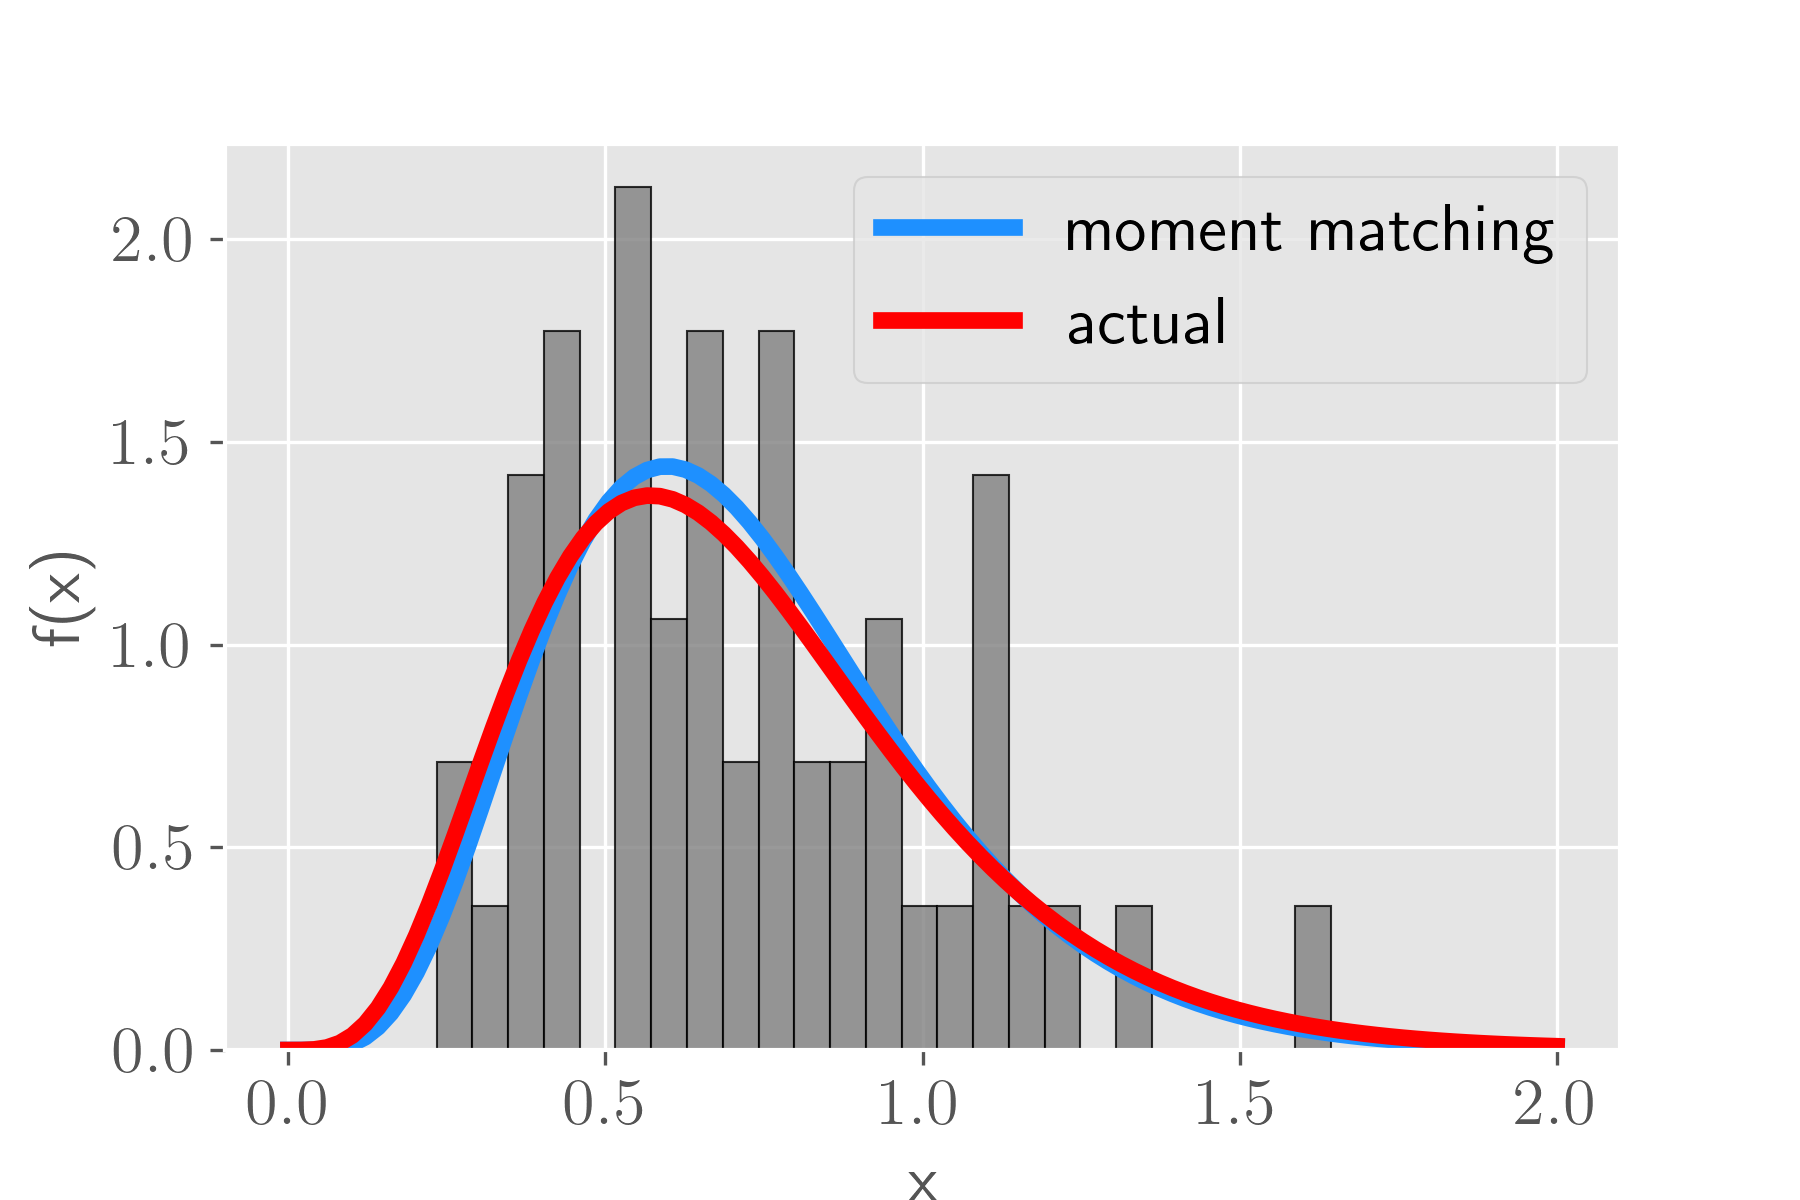
\includegraphics[scale=.7]{homework_1/first_hist.png}
    \caption{Estimated and actual densities with $\alpha = 5$, $\beta = 7$}
    \label{fig:my_label}
\end{figure}


\begin{figure}[!h]
    \centering
    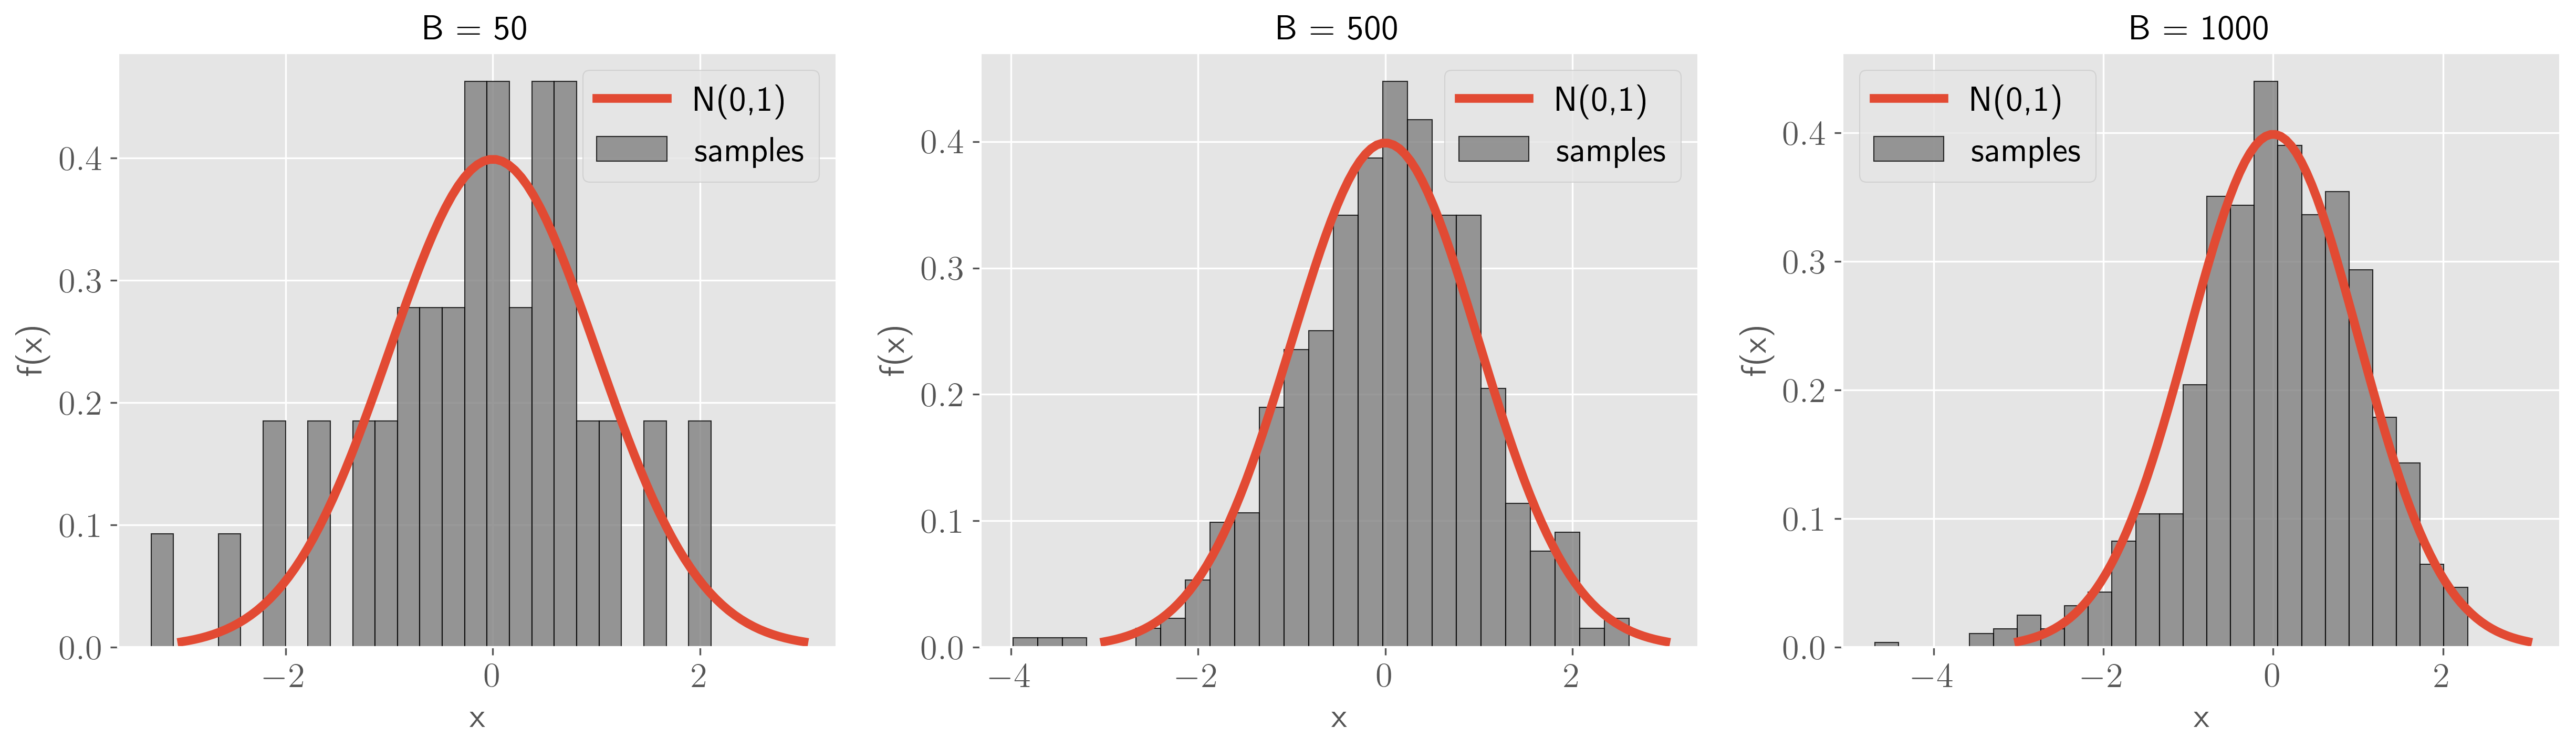
\includegraphics[scale=.35]{homework_1/second_hist.png}
    \caption{Samples and N(0,1)}
    \label{fig:my_label}
\end{figure}
\newpage
The first figure shows that the density estimated using moment matching is close to the actual one. Increasing the number of samples would improve the estimated density. The second figure confirms that the standard error derived for the estimator $\hat{\alpha}_n$ is $\sqrt{\frac{2\alpha(\alpha+1)}{n}}$; as $B$ increases the samples look more and more like the $N(0,1)$ density. $n = 50$ seems to be sufficiently high.

\section*{(6) For a Normal($\mu$, $\sigma^2$)
distribution, show that the MGF is $M(t) =\text{exp}(\mu t + \sigma^2t^2/2)$}


\begin{align*}
    M(t) &= E(e^{ty})\\
     &=\int_{-\infty}^{\infty} \text{exp}(ty)f(y)dt\\
     &= \int_{-\infty}^{\infty} \text{exp}(ty) \frac{1}{\sqrt{2\pi}\sigma}\text{exp}\left[ -\frac{1}{2}\left(\frac{y-\mu}{\sigma} \right )^2\right]
\end{align*}
Let $z = \left(\frac{y-\mu}{\sigma} \right )$; $dz/dy = 1/\sigma$.

\begin{align*}
    M(t) &= \int_{-\infty}^{\infty} \text{exp}(ty) \frac{1}{\sqrt{2\pi}\sigma}\text{exp}\left[ -\frac{1}{2}z^2\right]\sigma dz\\
    &= \int_{-\infty}^{\infty} \text{exp}(t[z\sigma+\mu]) \frac{1}{\sqrt{2\pi}\sigma}\text{exp}\left[ -\frac{1}{2}z^2\right]\sigma dz\\
    &=  \frac{1}{\sqrt{2\pi}} \int_{-\infty}^{\infty}  \text{exp}\left[ -\frac{1}{2}z^2+t(z\sigma+\mu)\right] dz\\
     &=  \frac{\text{exp}(\mu t)}{\sqrt{2\pi}} \int_{-\infty}^{\infty}  \text{exp}\left[ -\frac{1}{2}(z^2-2z\sigma t + \{\sigma t\}^2 - \{\sigma t\}^2 )\right] dz\\
         &=  \frac{\text{exp}(\mu t + \sigma^2t^2/2)}{\sqrt{2\pi}} \int_{-\infty}^{\infty}  \text{exp}\left[ -\frac{1}{2}(z^2-2z\sigma t + \{\sigma t\}^2 - \{\sigma t\}^2 )\right] dz\\
          &=  \text{exp}(\mu t + \sigma^2t^2/2) \int_{-\infty}^{\infty}  \frac{1}{\sqrt{2 \pi }} \text{exp}\left[ -\frac{1}{2}(z- \sigma t )^2\right] dz\\
           &=  \text{exp}(\mu t + \sigma^2t^2/2)
\end{align*}

Recognizing that the term inside the integral is the density of $N(\sigma t, 1)$.


\section*{(7) Show that a binomial random variable $R$ with denominator $m$ and probability $\pi$ has a cumulant generating function $K(t)=mlog(1-\pi+\pi e^t)$. Find lim K(t) as $m \rightarrow \infty$,  $\pi \rightarrow 0$ in a way so that $m\pi \rightarrow \lambda > 0$. Show that $Pr(R=r) \rightarrow \lambda^re^{-\lambda}/r!$ and hence establish that $R \xrightarrow[]{D} \text{Poisson}(\lambda)$. Using your favorite programming language, provide a numerical illustration of the result.}

Start with finding the MGF for a binomial distribution:

\begin{align*}
    MGF_r(t) &= \sum_{0}^{m}{m \choose r} \pi^r (1-\pi)^{m-r}e^{tr}\\
    &= \sum_{0}^{m}{m \choose r} (\pi e^t)^r (1-\pi)^{m-r}
\end{align*}

Using the binomial theorem:


\begin{align*}
    (x+y)^n = \sum_{0}^{n} {n \choose k} x^{n-k}y^k
\end{align*}

We find 

\begin{align*}
    MGF_r(t) &= (1-\pi+\pi e^t)^m
\end{align*}

So 

\begin{align*}
   K(t) &= \text{log}[MGF_r(t)]\\
   &=\text{log}[(1-\pi+\pi e^t)^m]\\
   &=m\text{log}(1-\pi+\pi e^t)
\end{align*}


Then, let $m\pi \to \lambda$,  $\lambda >0$

\begin{align*}
    \lim_{\substack{m\to\infty\\ \pi\to0}} K(t) & =  \lim_{\substack{m\to\infty\\ \pi\to0}} \text{log}[(1-\pi+\pi e^t)^m] \\
    &= \lim_{\substack{m\to\infty\\ \pi\to0}} \text{log}[\{1+\lambda / m (e^t-1)\}^m] \\
    &= \lambda(1-e^t)
\end{align*}
Using the hint given with $x\equiv \lambda(1-e^t)$. This corresponds to $MGF_r(t) = e^{\lambda(1-e^t)}$. Now, let's check that this corresponds to the MGF of $ \lambda^re^{-\lambda}/r!$, which is the pmf of the Poisson distribution.


\begin{align*}
    MGF_r(t) &=  \sum_{r=0}^{\infty} \frac{\lambda^Re^{-\lambda}}{r!}e^{tr}\\
    &=  \sum_{r=0}^{\infty} \frac{(\lambda t)^r e^{-\lambda}}{r!}
\end{align*}
Using $\sum a^x/x! = e^a$
\begin{align*}
    MGF_r(t) &= e^{-\lambda} e^{\lambda e^t}\\
    &= e^{\lambda(e^t-1)}
\end{align*}

The two MGF match, so $r \xrightarrow[]{D}
\text{Poisson}(\lambda)$.


\begin{figure}[!h]
    \centering
    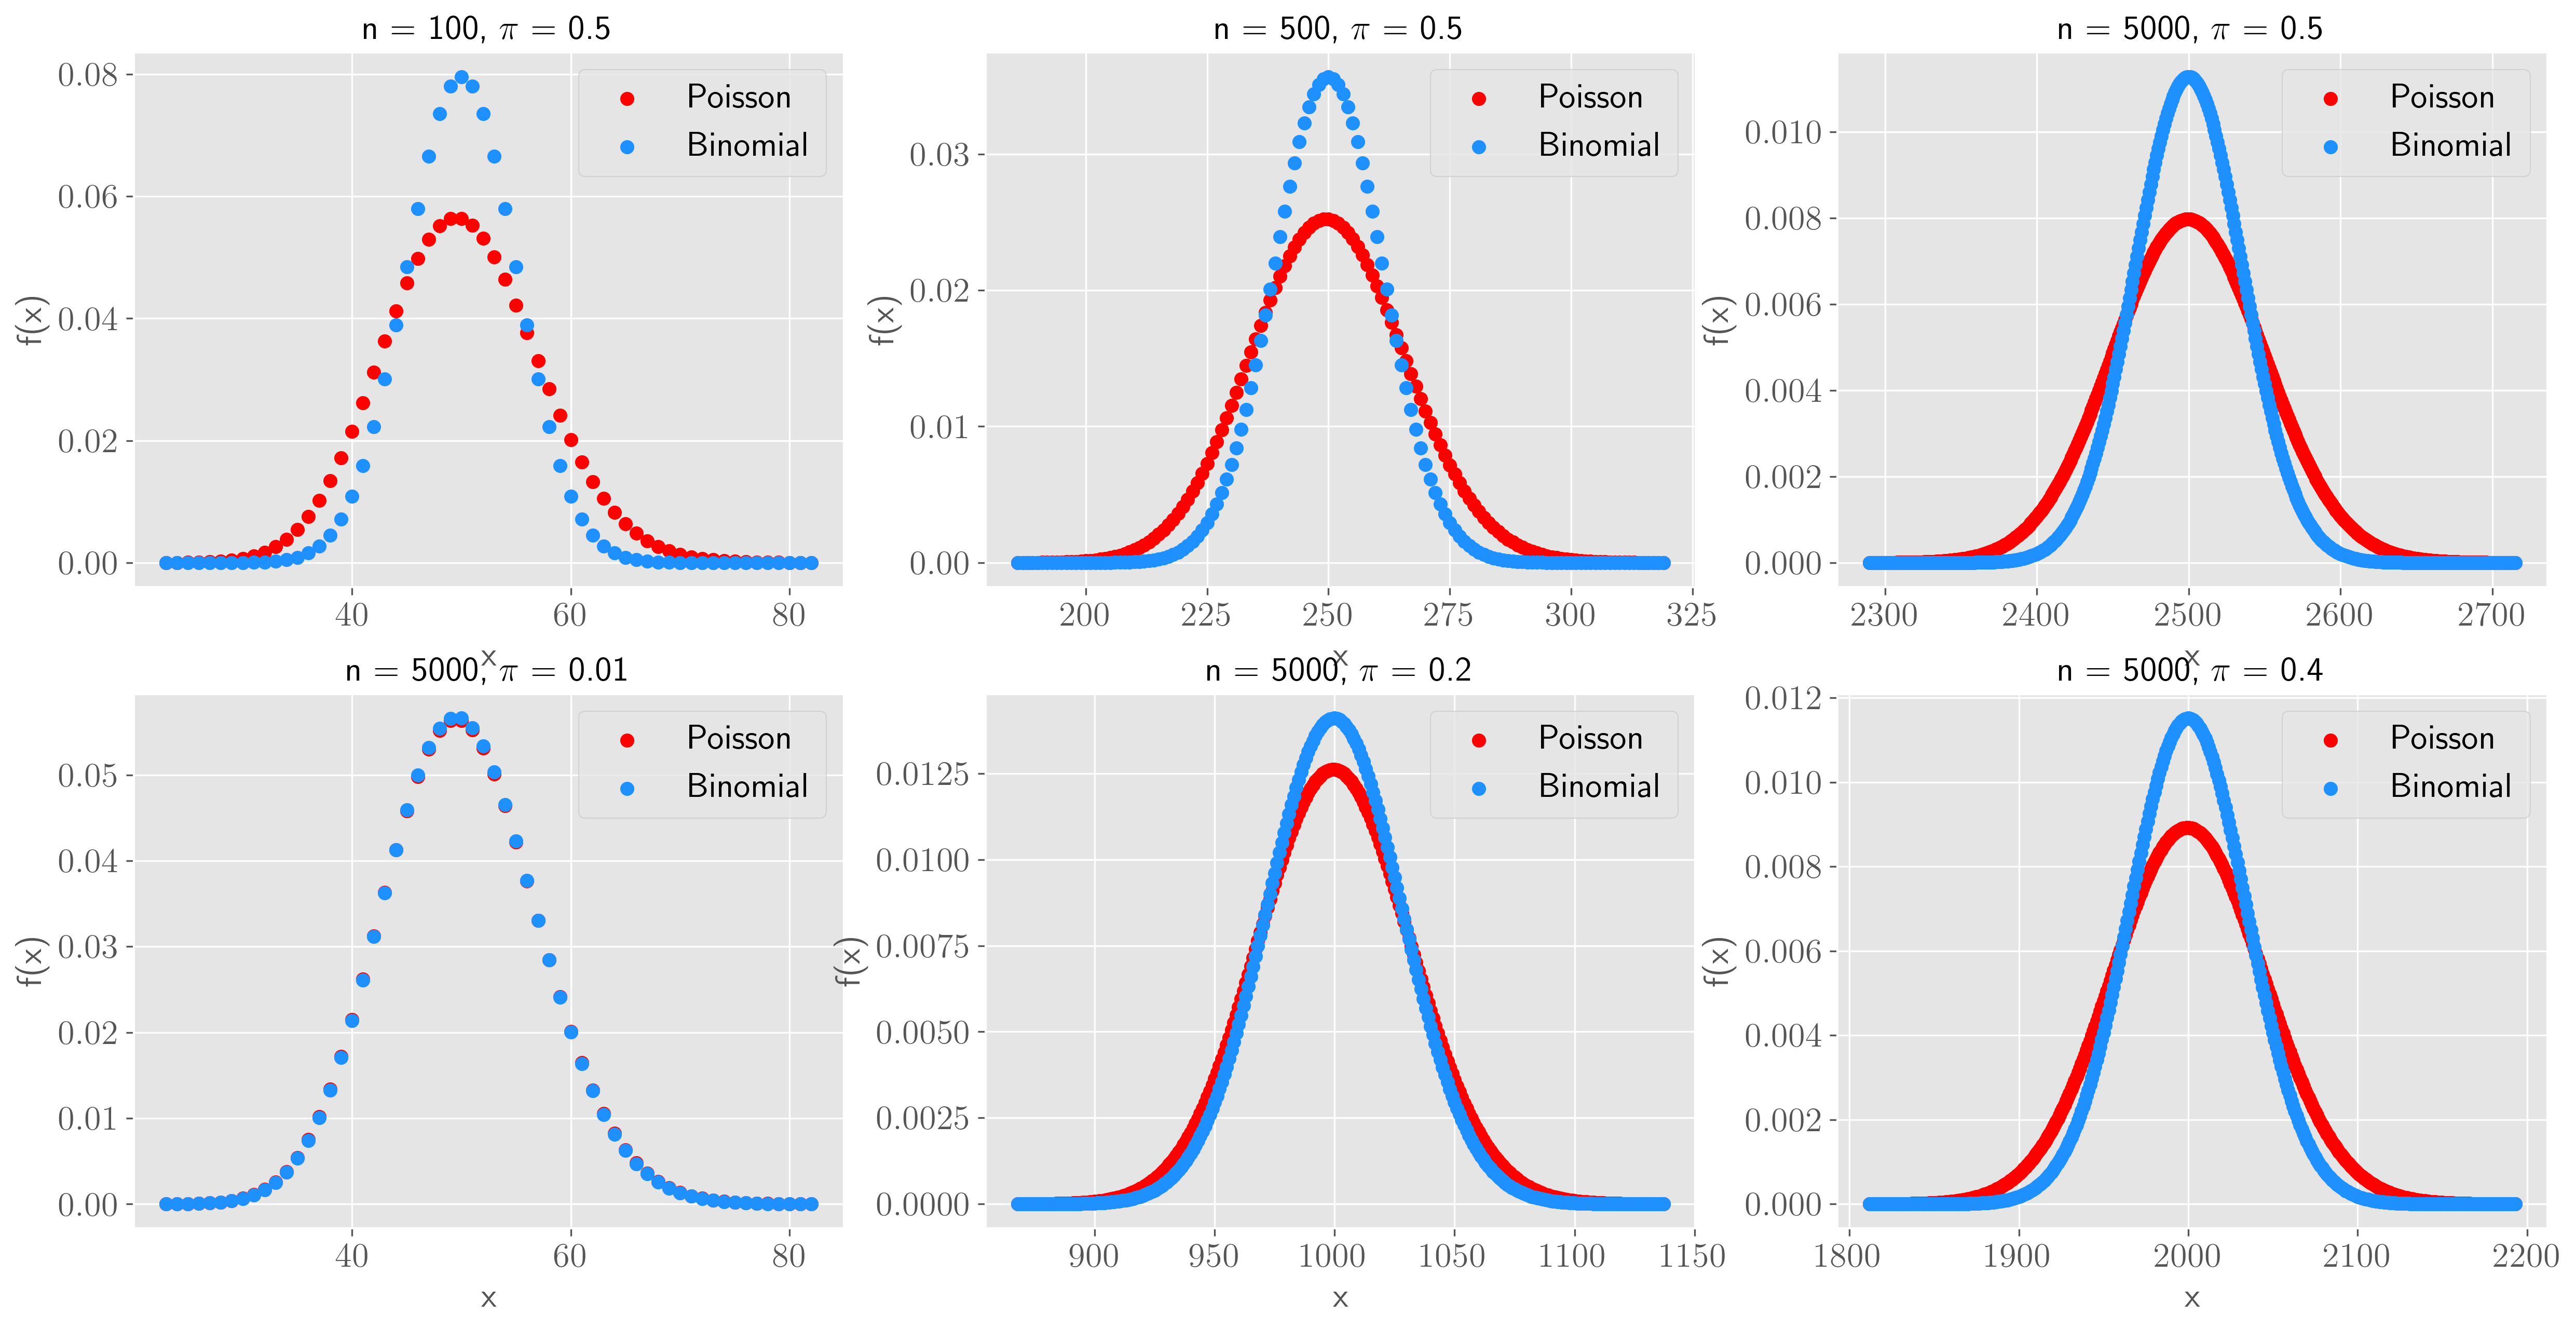
\includegraphics[scale=.35]{homework_1/third_hist.png}
    \caption{Illustration for binomial becoming Poisson at $\pi$ becomes small and $m$ is large.}
    \label{fig:my_label}
\end{figure}


\section*{(8) If $Z \sim N(0, 1)$, derive the density of $Y=Z^2$. Although Y is
determined by $Z$, show that they are uncorrelated.}
We will prove that $Y \sim \chi^2_1$ by showing that the $MGF$ of $Y$ is the same as that of the $\chi^2_1$ distribution.




 \begin{align*}
     MGF_y(t) &= \int_{-\infty}^{\infty} \frac{1}{\sqrt{2\pi}}e^{-y^2/2}e^{ty}dy\\
     &= \int_{-\infty}^{\infty} \frac{1}{\sqrt{2\pi}}e^{-(y^2/2)(1-2t)}dy\\
     &= (1-2t)^{-1/2}\int_{-\infty}^{\infty} \frac{1}{\sqrt{2\pi}(1-2t)^{-1/2}}e^{-(y^2/2)(1-2t)}dy\\
     &= (1-2t)^{-1/2}
 \end{align*}
 
 By recognizing the pdf of $N(0, \{1-2t\}^{-1})$. Now we obtain the MGF of $\chi^2_1$ using its pdf:
 
  \begin{align*}
     MGF_y(t) &=   \int_{-\infty}^{\infty} \frac{1}{\sqrt{2}\Gamma(1/2)} y^{-1/2}e^{-y/2}e^{ty}dy\\
     &=  \int_{-\infty}^{\infty} \frac{1}{\sqrt{2}\Gamma(1/2)} y^{-1/2}e^{-y/2(1-2t)}dy
 \end{align*}
 
 Let $\Tilde{y} = y(1-2t)$, so $dy/d\Tilde{y} = (1-2t)^{-1}$
 
   \begin{align*}
     MGF_y(t) &=  \int_{-\infty}^{\infty} \frac{1}{\sqrt{2}\Gamma(1/2)} [\Tilde{y}(1-2t)^{-1}]^{-1/2}e^{-\Tilde{y}/2}(1-2t)^{-1}d\Tilde{y}\\
     &=  (1-2t)^{-1/2} \int_{-\infty}^{\infty} \frac{1}{\sqrt{2}\Gamma(1/2)} \Tilde{y}^{-1/2}e^{-\Tilde{y}/2}d\Tilde{y}\\
      &=  (1-2t)^{-1/2}
 \end{align*}
From recognizing the pdf of  $\chi^2_1$ which integrates to 1. Since the two MGFs are the same, we have $Y \sim \chi^2_1$. Now we show that $cov(Y, Z)=0$.

\begin{align*}
    cov(Y, Z) &= E(YZ) - E(Z)E(Y)\\
    &= E(Z^3) - E(Z)E(Y)\\
    &= 0 - 0 \cdot 1\\
    &= 0
\end{align*}

We use the fact that $E(Z) = 0$ and that the skewness of $Z$ is 0; this can be shown using the third derivative of the MGF of $Z$.



\section*{(9) Let $Y = X_1 + bX_2$ where the $X_j$ are independent normals with means $\mu_j$ and variances $\sigma^2_j$ . Show that conditional on $X_2 = x$, the distribution of $Y$ is normal
with mean $\mu_1 + bx$ and variance $\sigma^2_1$.}

We start by finding the MGF of $\mu_1 + bx$, where $x$ is a fixed scalar. 

\begin{align*}
    MFG_y(t) &= E[e^{yt}] \\
    &=  E[e^{(X_1+bx)t}] \\ 
    & = e^{bxt}E[e^{X_1t}]\\
\end{align*}

Since $X_1$ is normally distributed with $\mu_1$ and $\sigma^2_1$, and we derived the MGF of the normal distribution earlier, we have: 

\begin{align*}
    MFG_y(t) &= e^{bxt}e^{\mu_1t + \sigma_1^2t^2/2}\\
    &= e^{(\mu_1 + bx)t + \sigma_1^2t^2/2}\\
\end{align*}

Which is the MGF of $\mathcal{N}(\mu_1 + bx, \sigma^2_1)$. So $(y|X_2=x) \sim \mathcal{N}(\mu_1 + bx, \sigma^2_1) $.

Then, we show that:

\begin{align*}
    \int \frac{1}{\sigma_1} \phi \left( \frac{y-\mu_1-bx}{\sigma_1}\right)  \frac{1}{\sigma_2} \phi \left( \frac{x-\mu_2}{\sigma_2}\right)dx = \frac{1}{\sqrt{\sigma^2_1+b^2\sigma^2_2}} \phi \left( \frac{y-\mu_1-b\mu_2}{{\sigma^2_1+b^2\sigma^2_2}}\right)
\end{align*}


\begin{align*}
    \int \frac{1}{\sigma_1}  \phi & \left( \frac{y-\mu_1-bx}{\sigma_1}\right)  \frac{1}{\sigma_2} \phi \left( \frac{x-\mu_2}{\sigma_2}\right)dx = \frac{1}{\sqrt{2\pi}\sigma_1} \frac{1}{\sqrt{2\pi}\sigma_2} \text{exp}\left(-\frac{1}{2}\frac{[y-\mu_1-bx]^2}{\sigma^2_1}\right)\left(-\frac{1}{2}\frac{[x-\mu_2]^2}{\sigma_2^2}\right)dx\\
    &= \int\frac{1}{\sqrt{2\pi}\sigma_1} \frac{1}{\sqrt{2\pi}\sigma_2} \text{exp}\left(-\frac{1}{2}\frac{[y-\mu_1-bx]^2}{\sigma^2_1}\right)\left(-\frac{1}{2}\frac{[x-\mu_2]^2}{\sigma_2^2}\right)dx\\
     &= \int\frac{1}{\sqrt{2\pi}\sigma_1} \frac{1}{\sqrt{2\pi}\sigma_2} \text{exp}\left(-\frac{1}{2}\frac{\sigma^2_2[y-\mu_1-bx]^2+\sigma^2_1[x-\mu_2]}{\sigma^2_1\sigma^2_2}\right)dx\\
      &= \int\frac{1}{\sqrt{2\pi}\sigma_1} \frac{1}{\sqrt{2\pi}\sigma_2} \text{exp}\left(-\frac{1}{2}\frac{\sigma^2_2[y-\mu_1-bx]^2+\sigma^2_1[x-\mu_2]}{\sigma^2_1\sigma^2_2}\right)dx\\
      &= \int\frac{1}{\sqrt{2\pi}\sigma_1} \frac{1}{\sqrt{2\pi}\sigma_2} \text{exp}\left(-\frac{1}{2}\frac{\sigma^2_2[y^2 + \mu_1^2 + b^2x^2 - 2y\mu_1 - 2ybx + 2\mu_1bx]+\sigma^2_1[x-2x\mu_2 + \mu_2^2]}{\sigma^2_1\sigma^2_2}\right)dx\\
      & = \int\frac{1}{\sqrt{2\pi}\sigma_1} \frac{1}{\sqrt{2\pi}\sigma_2} \text{exp}\left(-\frac{1}{2}\frac{x^2[\sigma^2_1+b^2\sigma^2_2]-2x[\sigma^2_2(by-b\mu_1)+\sigma^2_1\mu^2_2] + \sigma^2_2[y^2+\mu_1-2y\mu_1]+\sigma^2_1\mu^2_2}{\sigma^2_1\sigma^2_2}\right)dx\\
         & = \int\frac{1}{\sqrt{2\pi}\sigma_1} \frac{1}{\sqrt{2\pi}\sigma_2} \text{exp}\left(-\frac{1}{2}\frac{x^2[\sigma^2_1+b^2\sigma^2_2]-2x[\sigma^2_2(by-b\mu_1)+\sigma^2_1\mu_2] + \sigma^2_2[y^2+\mu_1-2y\mu_1]+\sigma^2_1\mu_2^2}{\sigma^2_1\sigma^2_2}\right)dx
\end{align*}

Let $\sigma^2 = \sigma^2_1+b^2\sigma^2_2$

\begin{align*}
 & = \int\frac{1}{\sqrt{2\pi}\sigma_1} \frac{1}{\sqrt{2\pi}\sigma_2} \text{exp}\left(-\frac{1}{2}\frac{x^2-\frac{2x[\sigma^2_2(by-b\mu_1)+\sigma^2_1\mu_2]}{{\sigma^2}} + \frac{ \sigma^2_2[y^2+\mu_1-2y\mu_1]}{{\sigma^2}}+\frac{\sigma^2_1\mu_2^2}{{\sigma^2}}}{\sigma^2_1\sigma^2_2/\sigma^2}\right)dx\\
 & =\int \frac{1}{\sqrt{2\pi}\sigma_1} \frac{1}{\sqrt{2\pi}\sigma_2} \text{exp}\left(-\frac{1}{2}\frac{\left\{x-\frac{[\sigma^2_2(by-b\mu_1)+\sigma^2_1\mu_2]}{{\sigma^2}}\right\}^2 -\left \{\frac{\sigma^2_2(by-b\mu_1)+\sigma^2_1\mu_2}{\sigma^2} \right \}^2 + \frac{ \sigma^2_2[y-\mu_1]^2}{{\sigma^2}}+\frac{\sigma^2_1\mu_2^2}{{\sigma^2}}}{\sigma^2_1\sigma^2_2/\sigma^2}\right)dx\\ 
 =\int \frac{1}{\sqrt{2\pi}\sigma_1}& \frac{1}{\sqrt{2\pi}\sigma_2} \text{exp}\left(-\frac{1}{2}\frac{\left\{x-\frac{[\sigma^2_2(by-b\mu_1)+\sigma^2_1\mu_2]}{{\sigma^2}}\right\}^2 }{\sigma^2_1\sigma^2_2/\sigma^2}\right) \\
 &\text{exp}\left(-\frac{1}{2}\frac{- [ \sigma^2_2b(y-\mu_1)+\sigma^2_1\mu_2]^2+ \sigma^2 (\sigma_2^2[y-\mu_1]^2+{\sigma^2_1\mu_2^2)}}{\sigma^2\sigma^2_1\sigma^2_2}\right)dx\\
\end{align*}


Let's focus on the term in the second exponential:
\begin{align*}
 &\frac{- [ \sigma^2_2b(y-\mu_1)+\sigma^2_1\mu_2]^2  + \sigma^2 (\sigma_2^2[y-\mu_1]^2+{\sigma^2_1\mu_2^2)}}{\sigma^2\sigma^2_1\sigma^2_2} \\ &= \frac{- [ \sigma^2_2b(y-\mu_1)+\sigma^2_1\mu_2]^2+ (\sigma^2_1+b^2 \sigma_2^2) (\sigma_2^2[y-\mu_1]^2+{\sigma^2_1\mu_2^2)}}{\sigma^2\sigma^2_1\sigma^2_2}\\
  &= \frac{- [ \sigma^4_2b^2(y-\mu_1)^2
  +2\sigma^2_2b(y-\mu_1)\sigma^2_1\mu_2+\sigma^4_1\mu_2^2]+ (\sigma^2_1+b^2 \sigma_2^2) (\sigma_2^2[y-\mu_1]^2+{\sigma^2_1\mu_2^2)}}{\sigma^2\sigma^2_1\sigma^2_2}\\
   &= \frac{(y-\mu_1)^2[-\sigma^4_2b^2+\sigma_1^2\sigma^2_2+b^2\sigma_2^4] - (y-\mu_1)[2\sigma_1^2\sigma_2^2b\mu_2]-\sigma_1^4\mu_2^2+\sigma_1^4\mu_2^2+b^2\sigma_1^2 \sigma_2^2\mu_2^2
}{\sigma^2\sigma^2_1\sigma^2_2}\\
   &= \frac{(y-\mu_1)^2 - 2b\mu_2(y-\mu_1)+b^2\mu_2^2
}{\sigma^2}\\
&= \frac{(y-[\mu_1+b\mu_2])^2 
}{\sigma^2}
\end{align*}

Going back and plugging in the term simplified above:
\begin{align*}
&=\int \frac{1}{\sqrt{2\pi}\sigma_1} \frac{1}{\sqrt{2\pi}\sigma_2} \text{exp}\left(-\frac{1}{2}\frac{\left\{x-\frac{[\sigma^2_2(by-b\mu_1)+\sigma^2_1\mu_2]}{{\sigma^2}}\right\}^2 }{\sigma^2_1\sigma^2_2/\sigma^2}\right) 
 \text{exp}\left(-\frac{1}{2} \frac{\{y-[\mu_1+b\mu_2]\}^2}{\sigma^2}\right)dx\\
 &=\int \frac{\sigma_1\sigma_2}{\sigma} \frac{\sigma}{\sigma_1\sigma_2 } \frac{1}{\sqrt{2\pi}\sigma_1} \frac{1}{\sqrt{2\pi}\sigma_2} \text{exp}\left(-\frac{1}{2}\frac{\left\{x-\frac{[\sigma^2_2(by-b\mu_1)+\sigma^2_1\mu_2]}{{\sigma^2}}\right\}^2 }{\sigma^2_1\sigma^2_2/\sigma^2}\right) 
 \text{exp}\left(-\frac{1}{2} \frac{\{y-[\mu_1+b\mu_2]\}^2}{\sigma^2}\right)dx\\
  &=  \frac{1}{\sqrt{2\pi}\sigma} 
 \text{exp}\left(-\frac{1}{2} \frac{\{y-[\mu_1+b\mu_2]\}^2}{\sigma^2}\right)\\
  &=  \frac{1}{\sqrt{2\pi}\sqrt{\sigma^2_1+b\sigma^2_2}} 
 \text{exp}\left(-\frac{1}{2} \frac{\{y-[\mu_1+b\mu_2]\}^2}{\sigma^2_1+b\sigma^2_2}\right)\\
   &=  \frac{1}{\sqrt{\sigma^2_1+b^2\sigma^2_2}} \phi \left( \frac{y-\mu_1-b\mu_2}{{\sigma^2_1+b^2\sigma^2_2}}\right)
 \end{align*}
 
Given that the distribution of the sum of two   independent random variables is the convolution of their individual distributions,
this gives us the pdf of $Y$, i.e. $Y \sim \mathcal{N}(\mu_1+b\mu_2, \mu_1^2+b^2\mu^2_2)$. 

\end{document}